\documentclass[titlepage]{article}
\usepackage{outline}
\usepackage{pmgraph}
\usepackage[normalem]{ulem}
\usepackage{comment} % enables the use of multi-line comments (\ifx \fi)
\usepackage{lipsum} %This package just generates Lorem Ipsum filler text.
%\usepackage{fullpage} % changes the margin
\usepackage{graphicx} % package for including images
\graphicspath{ {images/} } % path of images
% \begin{figure}[h]
% \includegraphics[width=8cm]{Plot}
% \end{figure}
\usepackage{geometry}
 \geometry{
 a4paper,
 left=20mm,
 top=1in,
 bottom=3in
 }
\title{\textbf{Lab 05: Simple Arithmetic Logic Unit}}
\author{Joseph Martinsen \\ ECEN 248-510 \\ TA: Michael Bass}
\date{\today}
%--------------------Make usable space all of page
\setlength{\oddsidemargin}{0in}
\setlength{\evensidemargin}{0in}
\setlength{\topmargin}{0in}
\setlength{\headsep}{-.25in}
\setlength{\textwidth}{6.5in}
\setlength{\textheight}{12in}
\linespread{1.5}
\setlength{\parindent}{4em}
\setlength{\parskip}{1em}

\usepackage{array}
\newcolumntype{L}[1]{>{\raggedright\let\newline\\\arraybackslash\hspace{0pt}}m{#1}}
\newcolumntype{C}[1]{>{\centering\let\newline\\\arraybackslash\hspace{0pt}}m{#1}}
\newcolumntype{R}[1]{>{\raggedleft\let\newline\\\arraybackslash\hspace{0pt}}m{#1}}
%--------------------Indention
\setlength{\parindent}{15pt}

\begin{document}
%--------------------Title Page
\maketitle



\section*{Objectives}
\hspace{15pt} The purpose of this lab was to design, implement, and test a simple
 4-bit Arithmetic Logic Unit (ALU) that has the ability to perform simple
 addition and subtraction. This lab also exposes the student to Two's Complement
 arithmetic and multiplexers.

\section*{Design}
\textbf{Experiment 1}
% hspace{15pt} for indent

 This lab had three seperate parts. The first part was modified
 from the initial lab desing to to the fact that there were not enough AND gates
 and XOR gates in order to create a 4 bit Ripple Carry Adder. Instead, the 4-bit
 adder IC was utilizied. Because of this, \textbf{Experiment 1} consisted of
 setting up the 4-bit IC to be connected to a DIP switch to supply the input,
 operants. Also the CIN was used as a \textbf{!Add/Sub} switch. The resulting
 4 bit sum was then displayed using four LEDs. The following is a desing of the
 Circuit that was built. \\
 \vspace{-30pt}
\begin{center}
  \begin{figure}[h]
    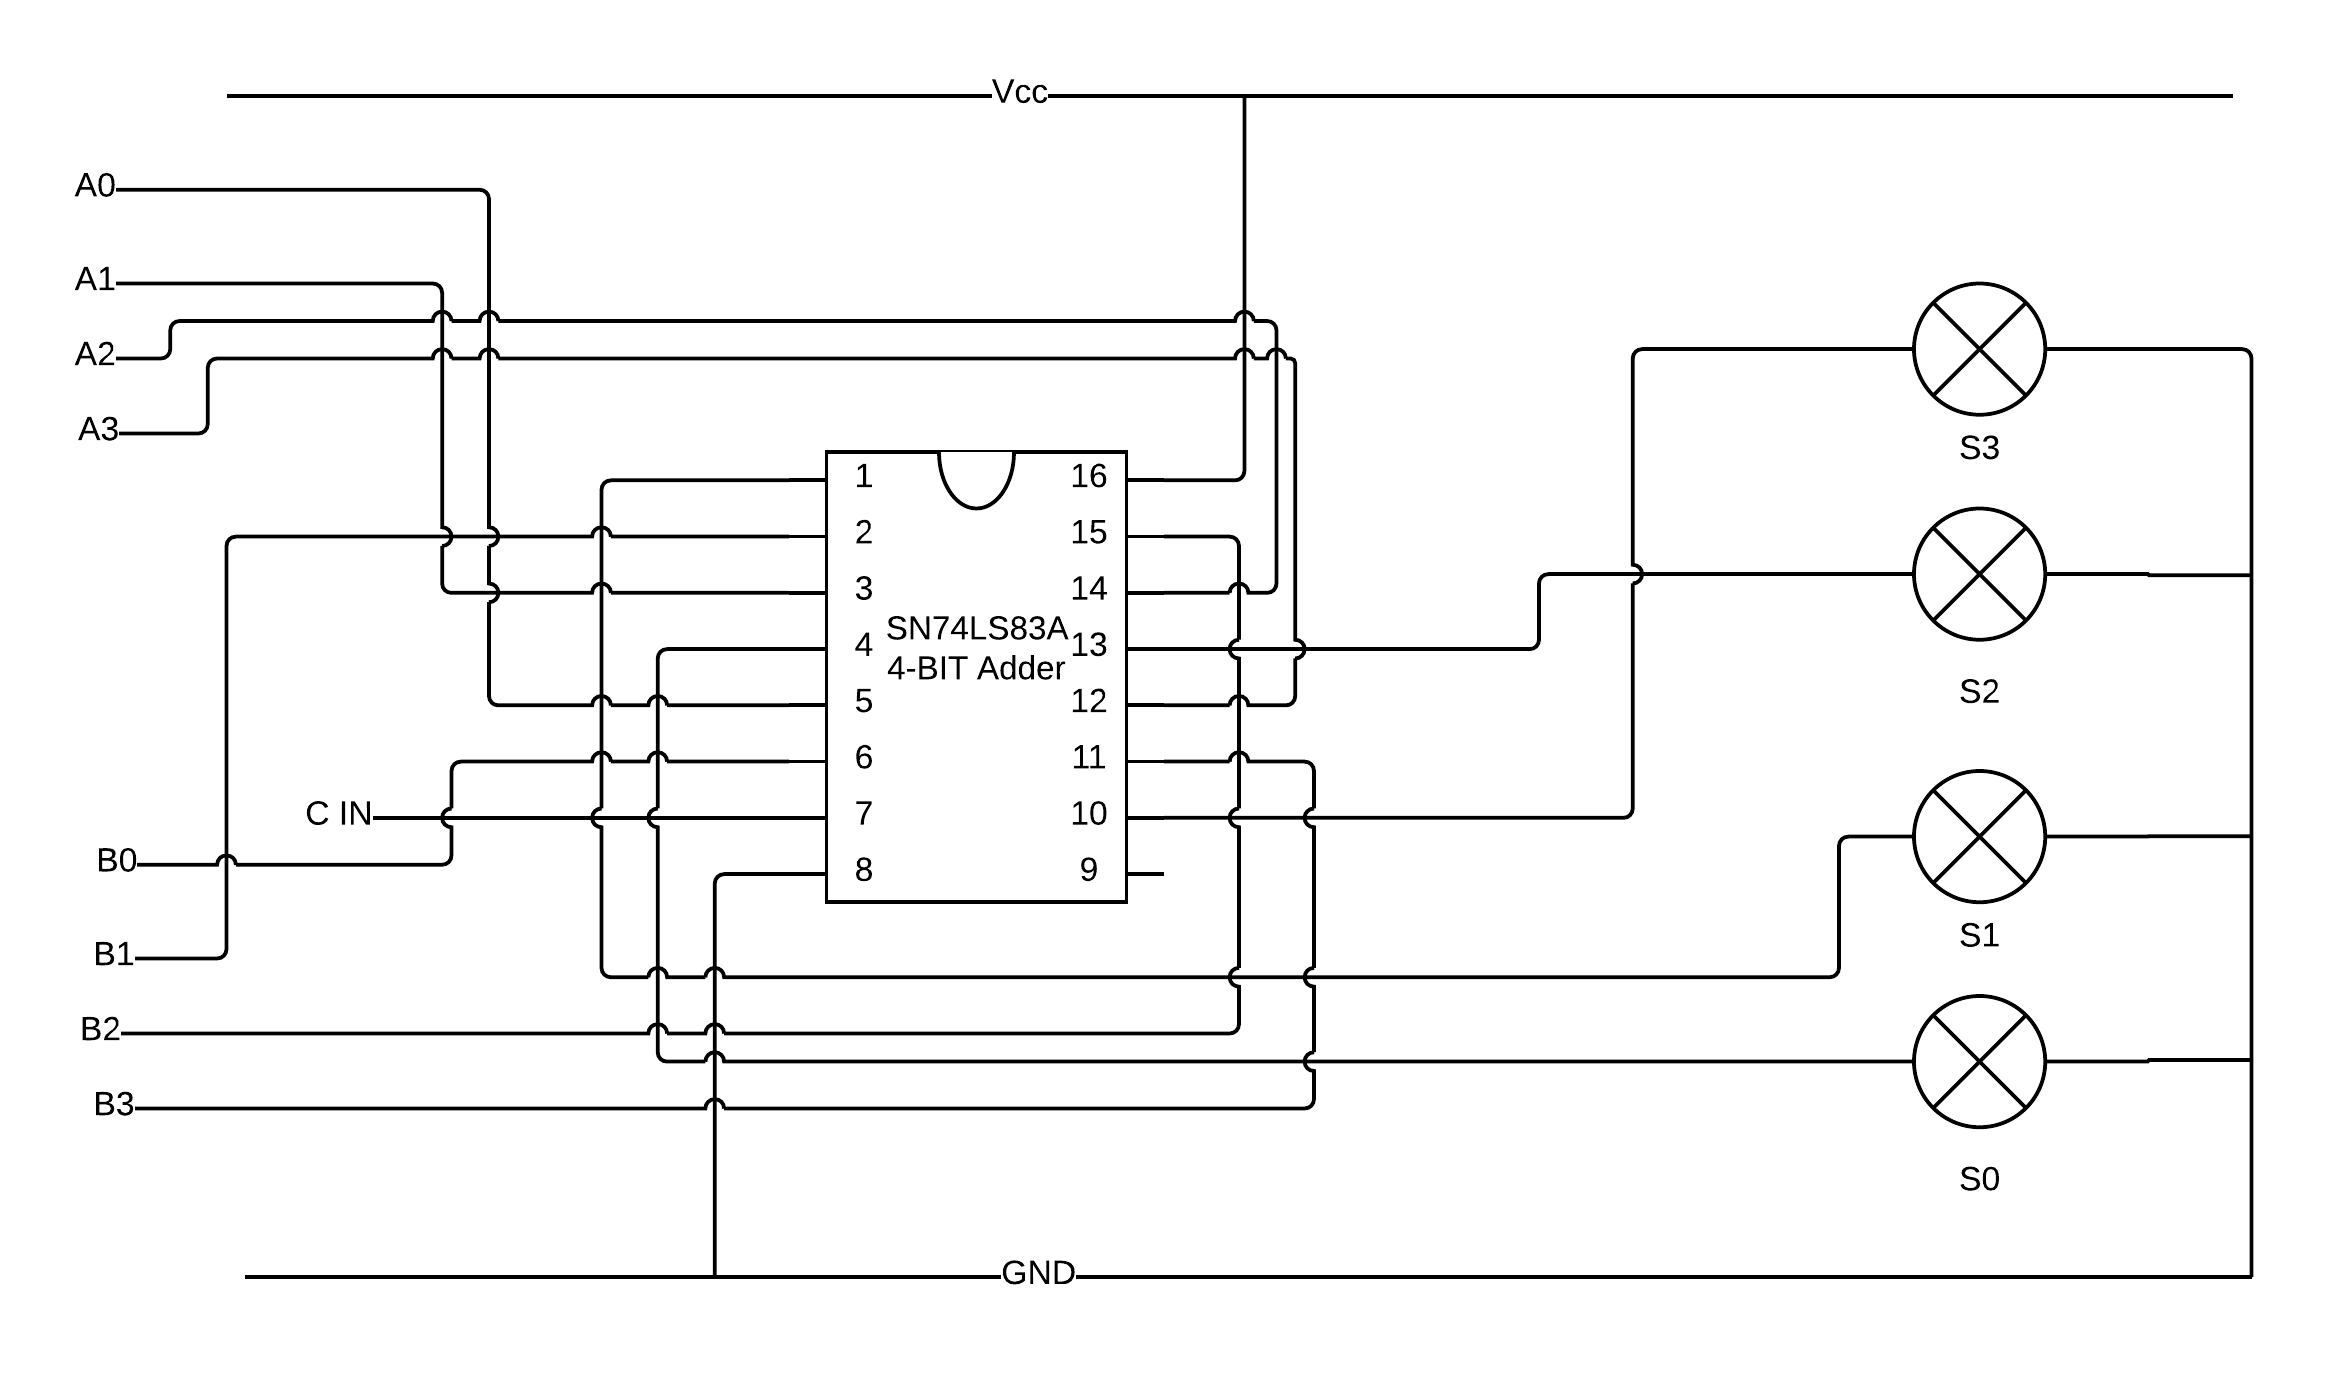
\includegraphics[scale=0.2]{4-BitAdder.png}
    \caption{\textit{4-Bit Adder Circuit}}
  \end{figure}
\end{center}
\vspace{-40pt}\textbf{Experiment 2}

 For the 2\textsuperscript{nd} expirement, on the same breadboard, a 2:1 MUX was
 used for the first time. The inputs \textit{A} and \textit{B} were hardwired for
 this part. The output was displayed on the LEDs. On the next page is a desing of the
 Circuit that was built. \\
 \vskip -1em
 \newpage
 \begin{figure}[h]
   \begin{center}
     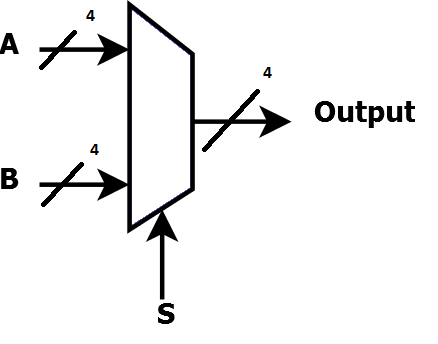
\includegraphics[scale=0.5]{4BitMux.png}
     \caption{\textit{4-Bit Mux}}
   \end{center}
 \end{figure}
\hspace{-15pt}\textbf{Experiment 3}

In the 3\textsuperscript{rd} and final part of the lab, the circuits built in
\textbf{Experiment 1} and \textbf{Experiment 2} \textit{(and shown in Fig 1 and Fig 2)}
were combined into one circuit. the outputs of \textbf{Experiment 1} were the
inputs of \textbf{Experiment 2}. The outputs of \textbf{Experiment 2} were then
connected to the LEDs. The inputs were hardwired for this part due to issues
with the DIP switch.\textbf{c1} and \textbf{c0} were also hardwired. The outputs
were then connected to 4 LED lights.
\vskip -1em

\section*{Results}

\textbf{Experiment 1}
% hspace{15pt} for indent

 This first part of the lab was able to be comleted rather quickly compared to
 having to build a 4-bit ripple adder. Due to the fact that we were using a 4-bit
 adder IC, it was not possible to XOR the values of the last two COUTs. The circuit
 was able to pass all the test values.\\
 \vskip -1em
\hspace{-15pt}\textbf{Experiment 2}

 For the 2\textsuperscript{nd} part, I encountered several issues setting up the
 None of the LEDs would turn on after the circuit was setup. I first used the
 multimeter to test to make sure that the power supply was outputing $5V$, which
 it was. I then checked to make sure the LEDs were recieving $5V$, which it was
 not. The LEDs were only getting $1.4V$. The issue was then somewhere in between the LEDs and power supply. I then
 checked the input values \textit{(A and B)} to make sure they were getting the
 correct voltage, which it was. I was able to find the culprit by testing the
 output of the MUX. The output was $1.4$, the same as the LEDs. I did not see
 anything wrong with the wiring so decided to replace the MUX IC. After the
 replacement, the circuit passed all the tests.\\
 \vskip -1em
\hspace{-15pt}\textbf{Experiment 3}

In the final part of the expirement, time became an issue. After constructing
the circuit, there was not much time left in lab and it took some time to setup
for each test case due to lack of orginaztion when combinging the MUX and the
4-bit adder. I believe that the circiut was setup and functiong properbly because
it passed the first three tests but due to time contraints, the final three tests
could not be checked.

\newpage

\section*{Conclution}

\hspace{15pt} In conclution, this lab taught me a lot on how multiplexors work as well how 4-bit
adders functions. I also learned how $2$'s complement is used in order to have
negative numbers in binary. I also learned, yet again, time contraints are a big
issue in these labs.
\section*{Questions}

\begin{enumerate}
  \item \textbf{Provide all design items found in the pre-lab deliverables.
  If you found that a design needed corrections while executing the lab, supply
   the updated version of that material.} \\
    \begin{figure}[h]
      \begin{center}
        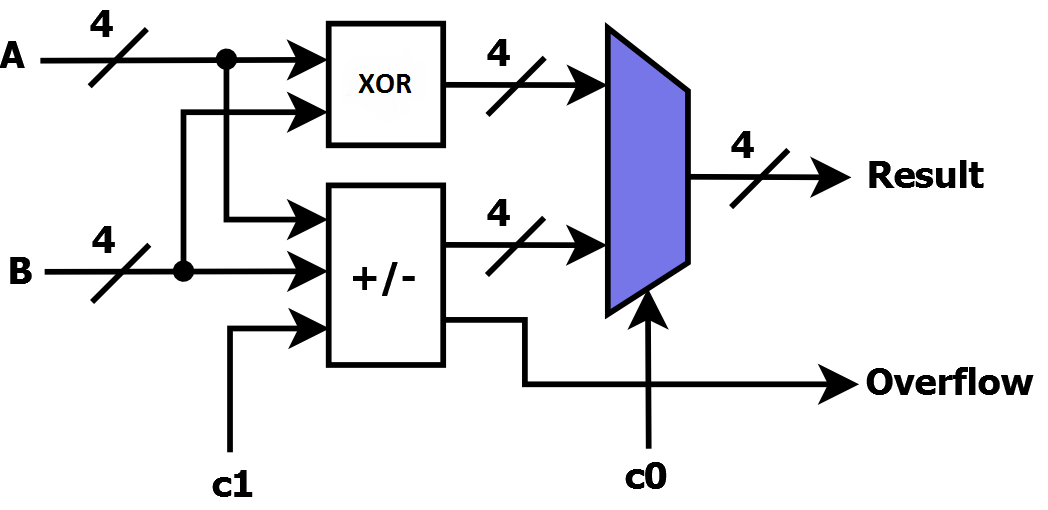
\includegraphics[scale=0.5]{ALUEdit.png}
      \end{center}
    \end{figure}
  \item \textbf{Create a table with the following columns: \textit{Control, A,
  B, Results} and \textit{Overflow.} Fill in sixteen rows of the table with with
  values from your bread-boaarded circuit, where twelve of the rows show the result
  of the addition/subtraction unit with at least two rows demonstrate overflow.} \\
  \begin{center}
    \begin{tabular}{|C{1.5cm}|C{1.5cm}|C{1.5cm}||C{1.5cm}| C{1.5cm}|}
      \hline
      \textit{Control} &\textit{A} & \textit{B} & \textit{Results} & \textit{Overflow} \\ [0.5ex]
      \hline
      \hline
      0 & 0 & 0 & 0 & 0 \\
      \hline
      0 & 0 & 1 & 1 & 0\\
      \hline
      0 & 1 & 0 & 1 & 0\\
      \hline
      0 & 1 & 1 & 0 & 1\\
      \hline
      \hline
       1 & 0 & 0 & 0 & 0\\
      \hline
       1 & 0 & 1 & 1 & 1\\
      \hline
       1 & 1 & 0 & 1 & 0\\
      \hline
       1 & 1 & 1 & 0 & 0\\
      \hline
    \end{tabular} \\ \ \\
    \textit{Not sure how to make 16 rows with only Control, A, and B}
  \end{center}

  \newpage

  \item \textbf{Determine the maximum gate delay through your final ALU circuit
  assuming each gate has a delay of 1 unit. Highlight the critical path on the
  gate-level schematic.} \\
    Using a 4 bit IC and a MUX, the delay would be only 2 units.

  \item \textbf{Draw a diagram showing how to construct an 8:1 multiplexer from
  4:1 and 2:1 multiplexers. Do \textbf{NOT} draw a gate-level schematic.} \\
  \begin{figure}[h]
    \begin{center}
      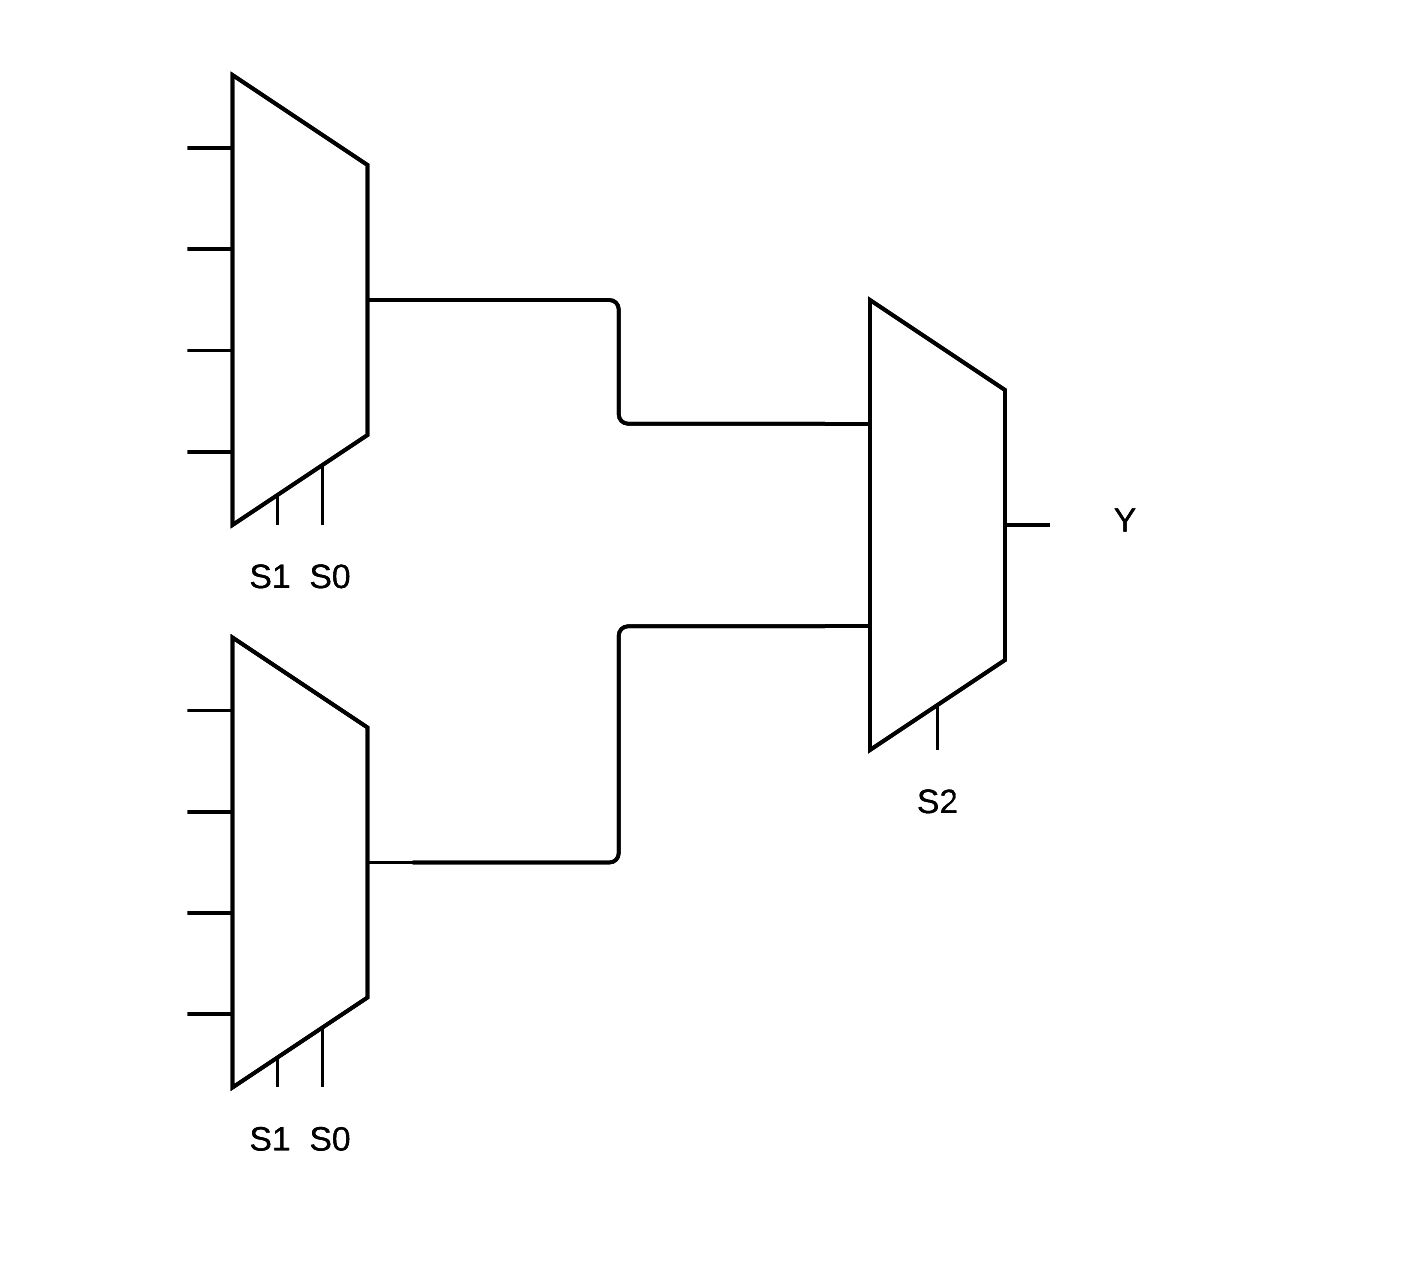
\includegraphics[scale=0.8]{8Mux.png}
    \end{center}
  \end{figure}

\end{enumerate}


\ifx
\section*{Attachments}
%Make sure to change these
Lab Notes, HelloWorld.ic, FooBar.ic
%\fi %comment me out

\begin{thebibliography}{9}
\bibitem{Robotics} Fred G. Martin \emph{Robotics Explorations: A Hands-On Introduction to Engineering}. New Jersey: Prentice Hall.
\bibitem{Flueck}  Flueck, Alexander J. 2005. \emph{ECE 100}[online]. Chicago: Illinois Institute of Technology, Electrical and Computer Engineering Department, 2005 [cited 30
August 2005]. Available from World Wide Web: (http://www.ece.iit.edu/~flueck/ece100).
\end{thebibliography}

%How to cite
Put your Problem statement here! Example of a Citation\cite[p.219]{Robotics}. Here's Another Citation\cite{Flueck}
\fi
\end{document}
